% !TeX program = xelatex
\documentclass[10pt]{beamer}

\usetheme{metropolis}

\usepackage{pgfplots}
\usepgfplotslibrary{fillbetween}
\usepackage{pgfopts}
\usepackage{amsmath}
\usepackage{structuralanalysis}
\usepackage{tikz}
\usepackage{tikz-3dplot}
\usepackage{chngcntr}
\usepackage{wasysym}
\usepackage{mathtools}
\usepackage{alphalph}
\usepackage{xcolor}
\usepackage[showdow=false, en-US]{datetime2}

\newcommand{\highlight}[1]{%
	\colorbox{red!50}{$\displaystyle#1$}}

\setcounter{lecture}{12}
\counterwithin{equation}{lecture}
\makeatletter
\def\user@resume{resume}
\def\user@intermezzo{intermezzo}
%
\newcounter{previousequation}
\newcounter{lastsubequation}
\newcounter{savedparentequation}
\setcounter{savedparentequation}{1}
% 
\renewenvironment{subequations}[1][]{%
	\def\user@decides{#1}%
	\setcounter{previousequation}{\value{equation}}%
	\ifx\user@decides\user@resume 
	\setcounter{equation}{\value{savedparentequation}}%
	\else  
	\ifx\user@decides\user@intermezzo
	\refstepcounter{equation}%
	\else
	\setcounter{lastsubequation}{0}%
	\refstepcounter{equation}%
	\fi\fi
	\protected@edef\theHparentequation{%
		\@ifundefined {theHequation}\theequation \theHequation}%
	\protected@edef\theparentequation{\theequation}%
	\setcounter{parentequation}{\value{equation}}%
	\ifx\user@decides\user@resume 
	\setcounter{equation}{\value{lastsubequation}}%
	\else
	\setcounter{equation}{0}%
	\fi
	\def\theequation  {\theparentequation  \alph{equation}}%
	\def\theHequation {\theHparentequation \alph{equation}}%
	\ignorespaces
}{%
%  \arabic{equation};\arabic{savedparentequation};\arabic{lastsubequation}
\ifx\user@decides\user@resume
\setcounter{lastsubequation}{\value{equation}}%
\setcounter{equation}{\value{previousequation}}%
\else
\ifx\user@decides\user@intermezzo
\setcounter{equation}{\value{parentequation}}%
\else
\setcounter{lastsubequation}{\value{equation}}%
\setcounter{savedparentequation}{\value{parentequation}}%
\setcounter{equation}{\value{parentequation}}%
\fi\fi
%  \arabic{equation};\arabic{savedparentequation};\arabic{lastsubequation}
\ignorespacesafterend
}
\makeatother
\title{AE 737 - Mechanics of Damage Tolerance}
\subtitle{Lecture \arabic{lecture}}
\date{Last Updated: \today\ at \DTMcurrenttime}
\author{Dr. Nicholas Smith}
\institute{Wichita State University, Department of Aerospace Engineering}
% \titlegraphic{\hfill\includegraphics[height=1.5cm]{logo/logo}}

\begin{document}

\maketitle
\begin{frame}{schedule}
	\begin{itemize}
		\item 1 Mar - Section 1 Review, Homework 5 Due
		\item 3 Mar - Section 1 Review, Homework 5 return
		\item 8 Mar - Exam 1
		\item 10 Mar - Exam return, Final Project discussion
	\end{itemize}
\end{frame}

\begin{frame}
  \frametitle{outline}
  \setbeamertemplate{section in toc}[sections numbered]
  \tableofcontents[hideallsubsections]
\end{frame}

\section{mixed mode fracture}

\begin{frame}{mixed-mode fracture}
	\begin{itemize}[<+->]
		\item Most cracks are primarily Mode I, but sometimes Mode II can also have an effect
		\item We can look at the combined stress field for Mode I and Mode II
		\item Recall the stress field near the crack tip
		\begin{subequations}
		\begin{align}
		\sigma_x &= \frac{K_I}{\sqrt{2\pi r}} \cos \frac{\theta}{2} \left(1-\sin \frac{\theta}{2}\sin \frac{3\theta}{2}\right)\\
		\sigma_y &= \frac{K_I}{\sqrt{2\pi r}} \cos \frac{\theta}{2} \left(1+\sin \frac{\theta}{2}\sin \frac{3\theta}{2}\right)\\
		\tau_{xy} &= \frac{K_I}{\sqrt{2\pi r}} \sin \frac{\theta}{2} \cos \frac{\theta}{2}\cos \frac{3\theta}{2}
		\end{align}
		\end{subequations}
	\end{itemize}
\end{frame}

\begin{frame}{mixed-mode fracture}
	\begin{itemize}[<+->]
		\item For Mode II we have
		\item[]
		\begin{subequations}
			\begin{align}
			\sigma_x &= \frac{-K_{II}}{\sqrt{2\pi r}} \sin \frac{\theta}{2} \left(2+\cos \frac{\theta}{2}\cos \frac{3\theta}{2}\right)\\
			\sigma_y &= \frac{K_{II}}{\sqrt{2\pi r}} \sin \frac{\theta}{2} \cos \frac{\theta}{2}\cos \frac{3\theta}{2}\\
			\tau_{xy} &= \frac{K_{II}}{\sqrt{2\pi r}} \cos \frac{\theta}{2} \left(1-\sin \frac{\theta}{2}\sin \frac{3\theta}{2}\right)
			\end{align}
		\end{subequations}
	\end{itemize}
\end{frame}

\begin{frame}{polar coordinates}
	\begin{itemize}[<+->]
		\item In mixed-mode fracture problems, the crack will generally propagate in a different direction from the initial crack plane
		\item It is more convenient to handle this scenario in Polar Coordinates
		\item We can convert stress from Cartesian coordinates to Polar Coordinates using the stress transformation equations
		\item[]
		\begin{subequations}
			\begin{align}
		\sigma_r &= \sigma_x \cos^2 \theta + \sigma_y \sin^2 \theta + 2\tau_{xy} \sin \theta \cos \theta\\
		\sigma_\theta &= \sigma_x \sin^2 \theta + \sigma_y \cos^2 \theta - 2\tau_{xy} \sin \theta \cos \theta\\
		\tau_{r\theta} &= -\sigma_x \sin \theta \cos \theta + \sigma_y \sin \theta \cos \theta + \tau_{xy} (\cos^\theta - \sin^2 \theta)
		\end{align}
		\end{subequations}
	\end{itemize}
\end{frame}

\begin{frame}{combined stress field}
	\begin{itemize}[<+->]
		\item When we convert the stress fields from Mode I and Mode II into polar coordinates and combine them, we find
		\item[]
		\begin{subequations}
			\begin{align}
			\sigma_r &= \frac{K_I}{\sqrt{2\pi r}} \left(\frac{5}{4}\cos \frac{\theta}{2} - \frac{1}{4}\cos \frac{3\theta}{2}\right) + \frac{K_{II}}{\sqrt{2\pi r}}\left(-\frac{5}{4}\sin \frac{\theta}{2} + \frac{3}{4}\sin \frac{3\theta}{2}\right)\\
			\label{eq:mixed-theta}
			\sigma_\theta &= \frac{K_I}{\sqrt{2\pi r}} \left(\frac{3}{4}\cos \frac{\theta}{2} + \frac{1}{4}\cos \frac{3\theta}{2}\right) + \frac{K_{II}}{\sqrt{2\pi r}}\left(-\frac{3}{4}\sin \frac{\theta}{2} - \frac{3}{4}\sin \frac{3\theta}{2}\right)\\
			\label{eq:mixed-tau}
			\tau_{r\theta} &= \frac{K_I}{\sqrt{2\pi r}} \left(\frac{1}{4}\sin \frac{\theta}{2} + \frac{1}{4}\sin \frac{3\theta}{2}\right) + \frac{K_{II}}{\sqrt{2\pi r}}\left(\frac{1}{4}\cos \frac{\theta}{2} + \frac{3}{4}\cos \frac{3\theta}{2}\right)
			\end{align}
		\end{subequations}
	\end{itemize}
\end{frame}

\begin{frame}{maximum circumferential stress criterion}
	\begin{itemize}[<+->]
		\item The Maximum Circumferential Stress Criterion assumes that a crack will propagate in the principal direction
		\item In this direction, the shear stress is 0
		\item The fracture toughness is determined by the Mode I fracture toughness of the material
		\item \textbf{Note:} In this discussion, we will use $K_{IC}$ to differentiate Mode I fracture toughness from Mode II fracture toughness. This does NOT necessarily mean we are referring to plane strain fracture toughness
		\item Thus fracture begins when
		\begin{equation}
		\sigma_{\theta}(\theta_P) = \sigma_\theta(\theta=0, K_{II}=0, K_I = K_{Ic}) = \frac{K_{IC}}{\sqrt{2\pi r}}
		\end{equation}
	\end{itemize}
\end{frame}

\begin{frame}{maximum circumferential stress criterion}
	\begin{itemize}[<+->]
		\item Following the above assumptions, we can solve Equations~\ref{eq:mixed-tau} and~\ref{eq:mixed-theta} to find $\theta_P$
		\item Note: This assumes that we know both $K_I$ and $K_{II}$, in this class we have not discussed any Mode II stress intensity factors, so they will be given.
		\item Equation~\ref{eq:mixed-tau} in this case simplifies to
		\begin{equation}
		K_I \sin \theta_p + K_{II} (3\cos \theta_P -1) = 0
		\end{equation}
		\item and Equation~\ref{eq:mixed-theta} simplifies to
		\begin{equation}
		4K_{IC} = K_I\left(3\cos \frac{\theta}{2} + \cos \frac{3\theta}{2}\right) - 3K_{II}\left(\sin \frac{\theta}{2} + \sin \frac{3\theta}{2}\right)
		\end{equation}
		\item The general form for a Mode II stress intensity factor is
		\item[]
		\begin{equation}
		K_{II} = \tau \sqrt{\pi a} \beta^\prime
		\end{equation}
	\end{itemize}
\end{frame}

\begin{frame}{example}
	\begin{figure}[H]
		Assuming $|\sigma| = 4|\tau|$, $K_{IC} = 60 \text{ ksi} \sqrt{\text{in}}$, and $2a = 1.5 \text{ in}$.
		
		\textbf{Note:} Assume $\beta = \beta^\prime = 1$
		
		\centering
		\begin{tikzpicture}
		\draw (0,-2) -- (0,2) -- (4,2) -- (4,-2) -- (0,-2);
		\draw (1.5,0) -- (2.5,0);
		\draw[->] (2,2.5) -- (2,3) node[above] {$\sigma$};
		\draw[->] (2,-2.5) -- (2,-3) node[below] {$\sigma$};
		\draw[->] (1,2.2) -- (3,2.2);
		\draw[->] (3,-2.2) -- (1,-2.2);
		\draw[->] (4.2,-1) -- (4.2,1);
		\draw[->] (-0.2,1) -- (-0.2,-1);
		\draw node at (4.2,2.2) {$\tau$};
		\draw node at (-0.2,-2.2) {$\tau$};
		\draw node at (2,0.2) {$2a$};
		\end{tikzpicture}
	\end{figure}
\end{frame}

\begin{frame}{principal stress criterion}
	\begin{itemize}[<+->]
		\item In the maximum circumferential stress criterion, we found the principal direction in polar coordinates
		\item We can also find the principal direction in Cartesian coordinates
		\item If we make a free body cut along some angle $\theta$ we find, from equilibrium
		\item[]
		\begin{subequations}
			\begin{align}
			0 &= \sigma_\theta dA - \sigma_x dA \sin^2 \theta - \sigma_y dA \cos^2 \theta + 2\tau_{xy} dA \cos \theta \sin \theta\\
			\sigma_\theta &= \sigma_x \sin^2 \theta + \sigma_y \cos^2 \theta - 2 \tau_{xy} \sin \theta \cos \theta\\
			\frac{\partial \sigma_\theta}{\partial \theta} &= (\sigma_x - \sigma_y) \sin 2\theta_p - 2\tau_{xy} \cos 2\theta_P\\
			\tan 2\theta_P &= \frac{2 \tau_{xy}}{\sigma_x - \sigma_y}
			\end{align}
		\end{subequations}
	\end{itemize}
\end{frame}

\begin{frame}{principal stress criterion}
	\begin{itemize}[<+->]
		\item As before, we consider crack propagation purely due to Mode I
		\item In the principal stress criterion, we find the maximum Mode I stress as a function of the remote applied stress
		\begin{equation}
		\sigma_{P1} = C \sigma
		\end{equation}
		\item We then find the remote failure stress by
		\begin{equation}
		\sigma_c = \frac{K_{IC}}{C\sqrt{\pi a}\beta}
		\end{equation}
	\end{itemize}
\end{frame}

\begin{frame}{example}
	\begin{figure}[H]
		Assuming $|\sigma| = 4|\tau|$, $K_{IC} = 60 \text{ ksi} \sqrt{\text{in}}$, and $2a = 1.5 \text{ in}$.
		
		\textbf{Note:} Assume $\beta = \beta^\prime = 1$
		
		\centering
		\begin{tikzpicture}
		\draw (0,-2) -- (0,2) -- (4,2) -- (4,-2) -- (0,-2);
		\draw (1.5,0) -- (2.5,0);
		\draw[->] (2,2.5) -- (2,3) node[above] {$\sigma$};
		\draw[->] (2,-2.5) -- (2,-3) node[below] {$\sigma$};
		\draw[->] (1,2.2) -- (3,2.2);
		\draw[->] (3,-2.2) -- (1,-2.2);
		\draw[->] (4.2,-1) -- (4.2,1);
		\draw[->] (-0.2,1) -- (-0.2,-1);
		\draw node at (4.2,2.2) {$\tau$};
		\draw node at (-0.2,-2.2) {$\tau$};
		\draw node at (2,0.2) {$2a$};
		\end{tikzpicture}
	\end{figure}
\end{frame}

\section{exam}

\begin{frame}{exam format}
	\begin{itemize}
		\item 4-5 questions
		\item Closed book, notes
		\item Equation sheet provided
		\item No T/F section, but the T/F questions in text can still be helpful
		\item Like homework, but simpler calculations
		\item In-class group review problems are also good practice for exam
	\end{itemize}
\end{frame}

\begin{frame}{overview}
	\begin{itemize}[<+->]
		\item Stress Intensity
		\begin{itemize}[<+->]
			\item Geometry-specific formulas
			\item Compounding
			\item Superposition
			\item Cracks on curved boundary
		\end{itemize}
	\end{itemize}
\end{frame}

\begin{frame}{overview}
	\begin{itemize}[<+->]
		\item Plastic Zone
		\begin{itemize}[<+->]
			\item Irwin's first approximation
			\item Irwin's correction
			\item Effective crack length
			\item Plane strain vs. plane stress
			\item Plastic zone shape
		\end{itemize}
	\end{itemize}
\end{frame}

\begin{frame}{overview}
	\begin{itemize}[<+->]
		\item Fracture Toughness
		\begin{itemize}[<+->]
			\item Plane strain fracture toughness - material property
			\item Plane stress fracture toughness - not
			\item Crack resistance curve
			\item General test/analysis methodology (ASTM)
			\item Thickness effects
		\end{itemize}
	\end{itemize}
\end{frame}

\begin{frame}{overview}
	\begin{itemize}[<+->]
		\item Residual Strength
		\begin{itemize}[<+->]
			\item Net section yield
			\item Fedderson
		\end{itemize}
	\end{itemize}
\end{frame}

\begin{frame}{overview}
	\begin{itemize}[<+->]
		\item Stiffeners
		\begin{itemize}[<+->]
			\item Panel, stiffener, rivet residual strength
			\item Positive slope in residual strength curve
			\item Analyze residual strength curves
		\end{itemize}
	\end{itemize}
\end{frame}

\begin{frame}{overview}
	\begin{itemize}[<+->]
		\item Multiple site damage
		\begin{itemize}[<+->]
			\item Link-up equation
			\item Modified link-up equation
			\item Ductile/tough vs. stiff/brittle materials
		\end{itemize}
	\end{itemize}
\end{frame}

\begin{frame}{overview}
	\begin{itemize}[<+->]
		\item Mixed-mode fracture
		\begin{itemize}[<+->]
			\item Maximum Circumferential Stress
			\item Principal Stress
			\item Why is principal stress method bad?
		\end{itemize}
	\end{itemize}
\end{frame}

\section{stress intensity}

\begin{frame}{compounding}
	\begin{itemize}
		\item Different types of boundaries create different correction factors to the usual stress intensity factor
		\item We often use $\beta$ to indicate the total correction factor
		\item When multiple boundaries are present, we can combine them into one effective correction factor
		\item There are two general methods we use to create a compound correction factor
	\end{itemize}
\end{frame}

\begin{frame}{compounding method 1}
	\begin{itemize}
		\item The first method uses linear superposition, and thus is restricted to cases where the effect of each boundary can be assumed to add linearly
		\item While in most cases this is not strictly true, it provides a reasonable approximation
		\begin{equation}
		K_r = \bar{K} + \sum_{i=1}^{N}(K_i - \bar{K})
		\end{equation}
		\item Where $N$ is the number of boundaries, $\bar{K}$ is the stress intensity factor with no boundaries present and $K_i$ is the stress intensity factor associated with the $i^{\text{th}}$ boundary.
	\end{itemize}
\end{frame}

\begin{frame}{compounding method 1}
	\begin{itemize}
		\item We can rewrite this equation as
		\begin{equation}
		K_r = \sigma \sqrt{\pi a} \beta_r = \sigma \sqrt{\pi a} + \sum_{i=1}^{N}(\sigma \sqrt{\pi a}\beta_i - \sigma \sqrt{\pi a})
		\end{equation}
		\item Which leads to an expression for $\beta_r$ as
		\begin{equation}
		\beta_r = 1+\sum_{i=1}^{N} (\beta_i - 1)
		\end{equation}
	\end{itemize}
\end{frame}

\begin{frame}{compounding method 2}
	\begin{itemize}
		\item An alternative empirical method approximates the boundary effect as
		\begin{equation}
		\beta_r = \beta_1 \beta_2 ... \beta_N
		\end{equation}
		\item If there is no interaction between the boundaries, method 1 and method 2 will give the same result
	\end{itemize}
\end{frame}

\begin{frame}{short cracks on curved boundaries}
	\begin{itemize}
		\item For short cracks, we can use the \emph{stress concentraction factor} on a curved boundary to determine the stress intensity factor
		\item The stress intensity factor only gives the maximum stress at the curved boundary, thus the longer the crack is, the farther away from the curved boundary (and maximum stress) it is.
	\end{itemize}
\end{frame}

\begin{frame}{short cracks on curved boundaries}
	\begin{itemize}
		\item Suppose we want to determine the stress intensity on a panel, panel B
		\item We find a similar panel with a known stress intensity factor, panel A
		\item We adjust the applied load on panel A such that $K_{I,A} = K_{I,B}$
		\item The magnitude of this load adjustment is determined using the \emph{stress concentration factors} in panels B and A
		\item Note the notation: $K_t$ for stress concentration factor, $K_I$ for stress intensity factor
	\end{itemize}
\end{frame}

\begin{frame}{short cracks on curved boundaries}
	\begin{figure}
		\begin{tikzpicture}
		\begin{scope}[scale=.75]
		\draw (0,-2.5) -- (0,2.5) -- (3,2.5) -- (3,-2.5) -- (0,-2.5);
		\draw[->] (1.5,2.5) -- (1.5,3) node[above] {$\sigma_B$};
		\draw[->] (1.5,-2.5) -- (1.5,-3) node[below] {$\sigma_B$};
		\draw (0.75,0) circle (0.5);
		\draw (.25,0) -- (0.15,0);
		\draw node at (1,-2) {$B$};
		\draw (5,-2.5) -- (5,2.5) -- (8,2.5) -- (8,-2.5) -- (5,-2.5);
		\draw[->] (6.5,2.5) -- (6.5,3) node[above] {$\sigma_A$};
		\draw[->] (6.5,-2.5) -- (6.5,-3) node[below] {$\sigma_A$};
		\draw (6.5,0) circle (0.5);
		\draw (6,0) -- (5.9,0);
		\draw node at (6,-2) {$A$};
		\end{scope}
		\end{tikzpicture}
	\end{figure}
\end{frame}

\begin{frame}{short cracks on curved boundaries}
	\begin{itemize}
		\item Since $A$ is a fictional panel, we set the applied stress, $\sigma_A$ such that
		\begin{equation*}
		\sigma_{max,B} = \sigma_{max,A}
		\end{equation*}
		\pause
		\item Substituting stress concentration factors
		\begin{equation*}
		K_{t,B} \sigma_B = K_{t,A} \sigma_A
		\end{equation*}
		\pause
		\item Solving for $\sigma_A$
		\begin{equation*}
		\sigma_A = \frac{K_{tB}}{K_tA}\sigma_B
		\end{equation*}
	\end{itemize}
\end{frame}

\begin{frame}{short cracks on curved boundaries}
	\begin{itemize}
		\item Since the crack is short and $\sigma_{max,A} = \sigma_{max,B}$ we can say
		\begin{align*}
		K_{I,B} &= K_{I,A}\\
		&= \sigma_A \sqrt{\pi c} \beta_A\\
		&= \frac{K_{t,B}}{K_{t,A}}\sigma_B \sqrt{\pi c} \beta_A
		\end{align*}
	\end{itemize}
\end{frame}

\begin{frame}<handout:0>{on-board example}
\end{frame}

\section{plastic zone}

\begin{frame}{Irwin's first approximation}
	\begin{figure}
		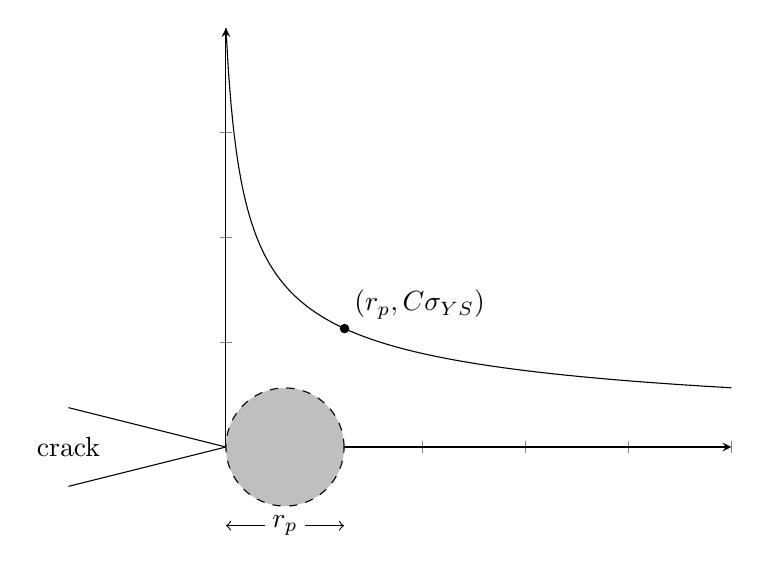
\begin{tikzpicture}
		\draw (-2,0.5) node at (-2,0) {crack} -- (0,0) -- (-2,-0.5);
		\begin{axis}[
		axis lines=middle,
		clip=false,
		ymin=0,
		xticklabels=\empty,
		yticklabels=\empty,
		cycle list name=black white,
		width=8cm,
		xmax=0.5,
		]
		\addplot+[mark=none,samples=200,unbounded coords=jump, domain=0.01:0.5] {1/sqrt(2*pi*x)};
		\draw[fill] (axis cs:0.125,1.128) circle [radius=1.5pt] node[above right] {$(r_p,C \sigma_{YS})$};
		\end{axis}
		\draw[dashed,fill=gray!50] (0.75,0) circle (0.75);
		\draw node at (0.75,-1) {$r_p$};
		\draw[->] (0.5,-1) -- (0,-1);
		\draw[->] (1,-1) -- (1.5,-1);
		\end{tikzpicture}
	\end{figure}
\end{frame}

\begin{frame}{Irwin's first approximation}
	\begin{itemize}
		\item We use $C$ "Plastic Constraint Factor" to convert between Plane Strain and Plane Stress solutions
		\item The plastic zone size can now be approximated by solving the equation $\sigma_{yy}(r=r_p) = C\sigma_{YS}$
		\pause
		\begin{subequations}
			\begin{align}
			\sigma_{yy}(r=r_p) &= C\sigma_{YS}\\
			\frac{K_I}{\sqrt{2\pi r_p}} &= C\sigma_{YS}\\
			r_p &= \frac{1}{2\pi} \left(\frac{K_I}{C\sigma_{YS}}\right)^2
			\end{align}
		\end{subequations}
	\end{itemize}
\end{frame}

\begin{frame}{Irwin's first approximation}
	\begin{itemize}
		\item For plane stress (thin panels) we let $C=1$ and find $r_p$ as
		\begin{equation}
		r_p = \frac{1}{2\pi} \left(\frac{K_I}{\sigma_{YS}}\right)^2
		\end{equation}
		\pause
		\item And for plane strain (thick panels) we let $C=\sqrt{3}$ and find
		\begin{equation}
		r_p = \frac{1}{6\pi} \left(\frac{K_I}{\sigma_{YS}}\right)^2
		\end{equation}
	\end{itemize}
\end{frame}

\begin{frame}{Intermediate panels}
	\begin{itemize}
		\item For panels which lie between plane strain and plane stress states, we use the following expression to estimate the plastic zone size
		\begin{equation}
		r_p = \frac{1}{I\pi} \left(\frac{K_I}{\sigma_{YS}}\right)^2
		\end{equation}
		\pause
		\item Where $I$ is defined as
		\begin{equation}
		I = 6.7 - \frac{1.5}{t}\left(\frac{K_I}{\sigma_{YS}}\right)^2
		\end{equation}
		\item And $2 \le I \le 6$
	\end{itemize}
\end{frame}

\begin{frame}{Irwin's second approximation}
	\begin{itemize}
		\item If our material is perfectly elastic-plastic, no stresses above $C\sigma_{YS}$ will exist in the material
		\item This ignores the strain energy (represented by the area under the curve) in the plastic zone
	\end{itemize}
\end{frame}

\begin{frame}{Irwin's second approximation}
	\begin{figure}
		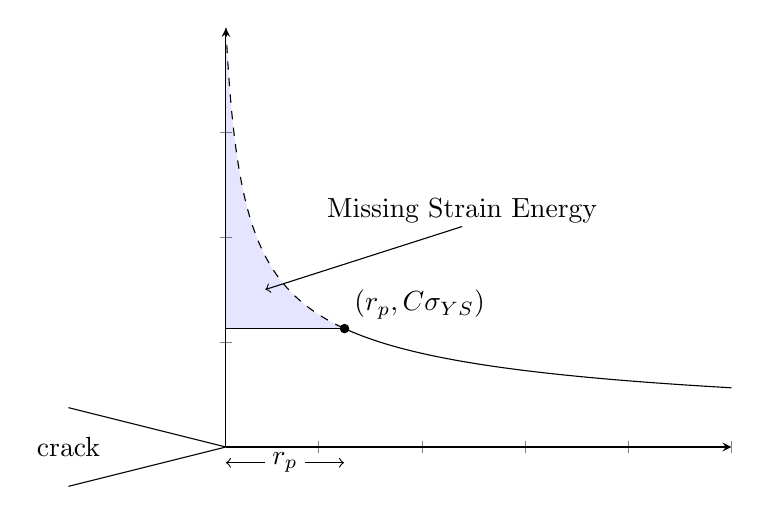
\begin{tikzpicture}
		\draw (-2,0.5) node at (-2,0) {crack} -- (0,0) -- (-2,-0.5);
		\begin{axis}[
		axis lines=middle,
		clip=false,
		ymin=0,
		xticklabels=\empty,
		yticklabels=\empty,
		cycle list name=black white,
		width=8cm,
		xmax=0.5,
		]
		\addplot[mark=none,samples=200,unbounded coords=jump, domain=0.125:0.5] {1/sqrt(2*pi*x)};
		\addplot[name path=a,mark=none,dashed,samples=200,unbounded coords=jump, domain=0.01:0.125] {1/sqrt(2*pi*x)};
		\addplot[name path=b,mark=none,samples=200,unbounded coords=jump, domain=0.01:0.125] {1/sqrt(2*pi*.125)};
		\addplot[fill=blue, fill opacity=.1] fill between[of=a and b];
		\draw[fill] (axis cs:0.125,1.128) circle [radius=1.5pt] node[above right] {$(r_p,C \sigma_{YS})$};
		\end{axis}
		\draw node at (0.75,-.2) {$r_p$};
		\draw[->] (0.5,-.2) -- (0,-.2);
		\draw[->] (1,-.2) -- (1.5,-.2);
		\draw node at (3,3) {Missing Strain Energy};
		\draw[->] (3,2.8) -- (0.5,2);
		\end{tikzpicture}
	\end{figure}
\end{frame}

\begin{frame}{Irwin's second approximation}
	\begin{itemize}
		\item To account for the additional strain energy, Irwin considered a plastic zone size increased by some $\delta$
		\item He also needed to adjust the stress function, and considered an equivalent crack tip in these calculations
	\end{itemize}
\end{frame}

\begin{frame}{Irwin's second approximation}
	\begin{figure}
		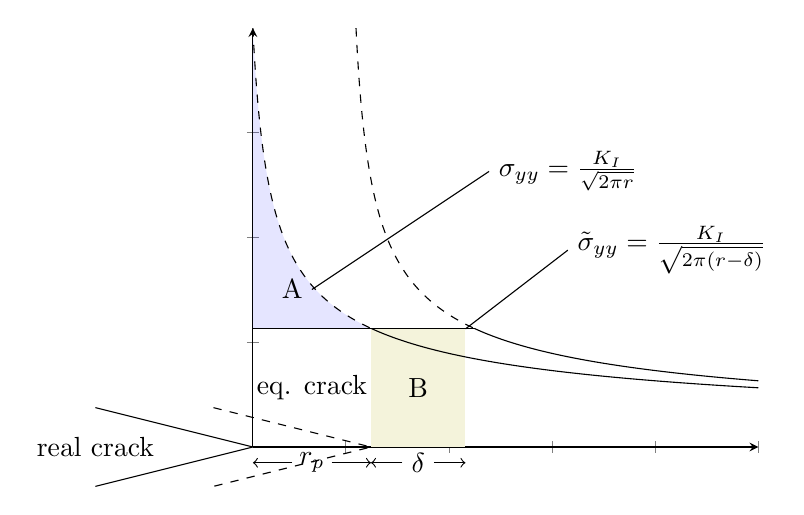
\begin{tikzpicture}
		\draw (-2,0.5) node at (-2,0) {real crack} -- (0,0) -- (-2,-0.5);
		\draw[dashed] (-.5,0.5) node at (.75,.75) {eq. crack} -- (1.5,0) -- (-.5,-0.5);
		\fill[olive!10] (1.5,0) rectangle (2.7,1.5);
		\begin{axis}[
		axis lines=middle,
		clip=false,
		ymin=0,
		xticklabels=\empty,
		yticklabels=\empty,
		cycle list name=black white,
		width=8cm,
		xmax=0.5,
		]
		\addplot[mark=none,samples=200,unbounded coords=jump, domain=0.125:0.5] {1/sqrt(2*pi*x)};
		\addplot[name path=a,mark=none,dashed,samples=200,unbounded coords=jump, domain=0.01:0.125] {1/sqrt(2*pi*x)};
		\addplot[name path=b,mark=none,samples=200,unbounded coords=jump, domain=0.01:0.225] {1/sqrt(2*pi*.125)};
		\addplot[fill=blue, fill opacity=.1] fill between[of=a and b];
		\addplot[name path=c,mark=none,dashed,samples=200,unbounded coords=jump, domain=0.11:0.225] {1/sqrt(2*pi*(x-.1))};
		\addplot[name path=d,mark=none,samples=200,unbounded coords=jump, domain=0.225:0.5] {1/sqrt(2*pi*(x-.1))};
		\end{axis}
		\draw node at (0.75,-.2) {$r_p$};
		\draw[->] (0.5,-.2) -- (0,-.2);
		\draw[->] (1,-.2) -- (1.5,-.2);
		\draw node at (2.1,-.2) {$\delta$};
		\draw[->] (2.3,-.2) -- (2.7,-.2);
		\draw[->] (1.9,-.2) -- (1.5,-.2);
		\draw[-] (3,3.5) node[right] {$\sigma_{yy} = \frac{K_I}{\sqrt{2\pi r}}$} -- (0.75,2);
		\draw[-] (4,2.5) node[right] {$\tilde{\sigma}_{yy} = \frac{K_I}{\sqrt{2\pi (r-\delta)}}$} -- (2.7,1.5);
		\draw node at (.5,2) {A};
		\draw node at (2.1,0.75) {B};
		\end{tikzpicture}
	\end{figure}
\end{frame}

\begin{frame}{Irwin's second approximation}
	\begin{itemize}
		\item We need $A=B$, so we set them equivalent and solve for $\delta$.
		\begin{subequations}
			\begin{align}
			A &= \int_{0}^{r_p} \sigma_{yy} dr - r_p \sigma_{YS}\\
			&= \int_{0}^{r_p} \frac{K_I}{\sqrt{2\pi r}} dr - r_p \sigma_{YS}\\
			&= \frac{K_I}{\sqrt{2\pi}}\int_{0}^{r_p} r^{-1/2} dr - r_p \sigma_{YS}\\
			&= \frac{2K_I \sqrt{r_p}}{\sqrt{2\pi}}- r_p \sigma_{YS}
			\end{align}
			\item We have already found $r_p$ as
			\begin{equation}
			r_p = \frac{1}{2\pi} \left(\frac{K_I}{\sigma_{YS}}\right)^2
			\end{equation}
			\item If we solve this for $K_I$ we find
			\begin{equation}
			K_I = \sqrt{2\pi r_p} \sigma_{YS}
			\end{equation}
		\end{subequations}
	\end{itemize}
\end{frame}

\begin{frame}{Irwin's second approximation}
	\begin{itemize}
		\item We can now substitute back into the strain energy of A
		\begin{subequations}[resume]
			\begin{align}
			A &= \frac{2\sqrt{2\pi r_p} \sigma_{YS} \sqrt{r_p}}{\sqrt{2\pi}}- r_p \sigma_{YS}\\
			&= 2 \sigma_{YS} r_p- r_p \sigma_{YS}\\
			&= r_p \sigma_{YS}
			\end{align}
			\item B is given simply as $B = \delta \sigma_{YS}$, so we equate A and B to find $\delta$
			\begin{align}
			A &= B\\
			r_p \sigma_{YS} &= \delta \sigma_{YS}\\
			r_p &= \delta
			\end{align}
		\end{subequations}
	\end{itemize}
\end{frame}

\begin{frame}{Irwin's second approximation}
	\begin{itemize}
		\item This means the plastic zone size is simply $2r_p$
		\item However, it also means that the effective crack length is $a + r_p$
		\pause
		\item Since $r_p$ depends on $K_I$, we must iterate a bit to find the "real" $r_p$ and $K_I$
	\end{itemize}
\end{frame}

\end{document}
